\documentclass{beamer}
%\beamerdefaultoverlayspecification{<+->}

\usetheme{metropolis}      % Use metropolis theme
\usepackage{graphicx}
\usepackage{amsmath}
\usepackage{mathtools}

\title{Neural Networks for Image Classification}
\date{\today}
\author{Catalina Vajiac}
\institute{Saint Mary's College}

\begin{document}
  \maketitle

  \section{Introduction}
  \begin{frame}{Overview}
    \begin{itemize}
      \item What is a neural network?
      \item Types of Neural Networks
      \begin{itemize}
        \item fully-connected
        \item deep
        \item convolutional
      \end{itemize}
      \item Gradient Descent
      \begin{itemize}
        \item Softmax classifier
        \begin{itemize}
          \item gradient derivation
        \end{itemize}
        \item single-layer neural network
      \end{itemize}
      \item Demonstration of Softmax classifier
      \begin{itemize}
        \item randomized tests
        \item MNIST Dataset
      \end{itemize}
    \end{itemize}
  \end{frame}

  \section{Neural Networks}
  \begin{frame}{What is a Neural Network?}
    \begin{itemize}
      \item collection of units (neurons) that transmit signals to one another
      \item each unit processes signal, propagates forward
      \item allows computer to learn from observational data
    \end{itemize}
    \begin{center}
      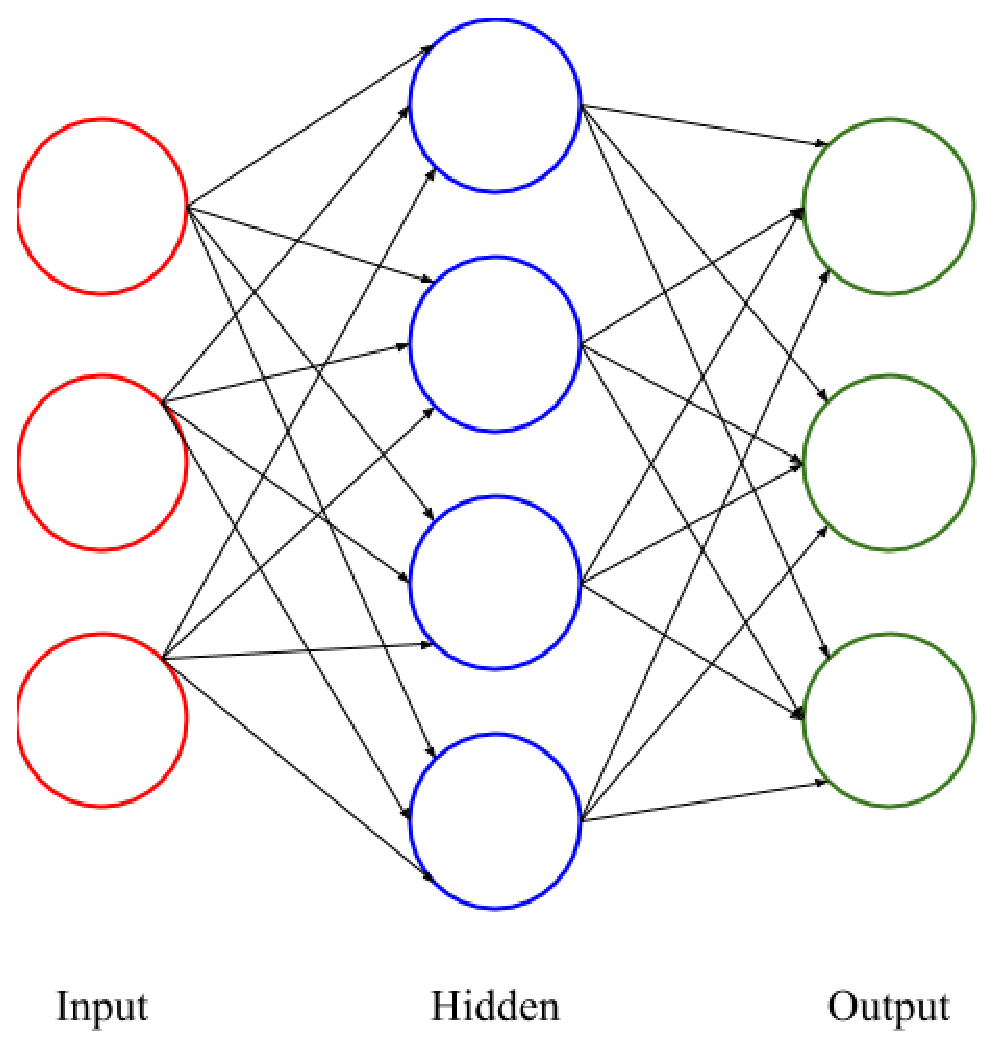
\includegraphics[height=2in]{../figures/neural_network.eps}
    \end{center}
  \end{frame}

  \section{Types of Neural Networks}
  \begin{frame}{Fully Connected Network}
    \begin{figure}[ht!]
      \centering
      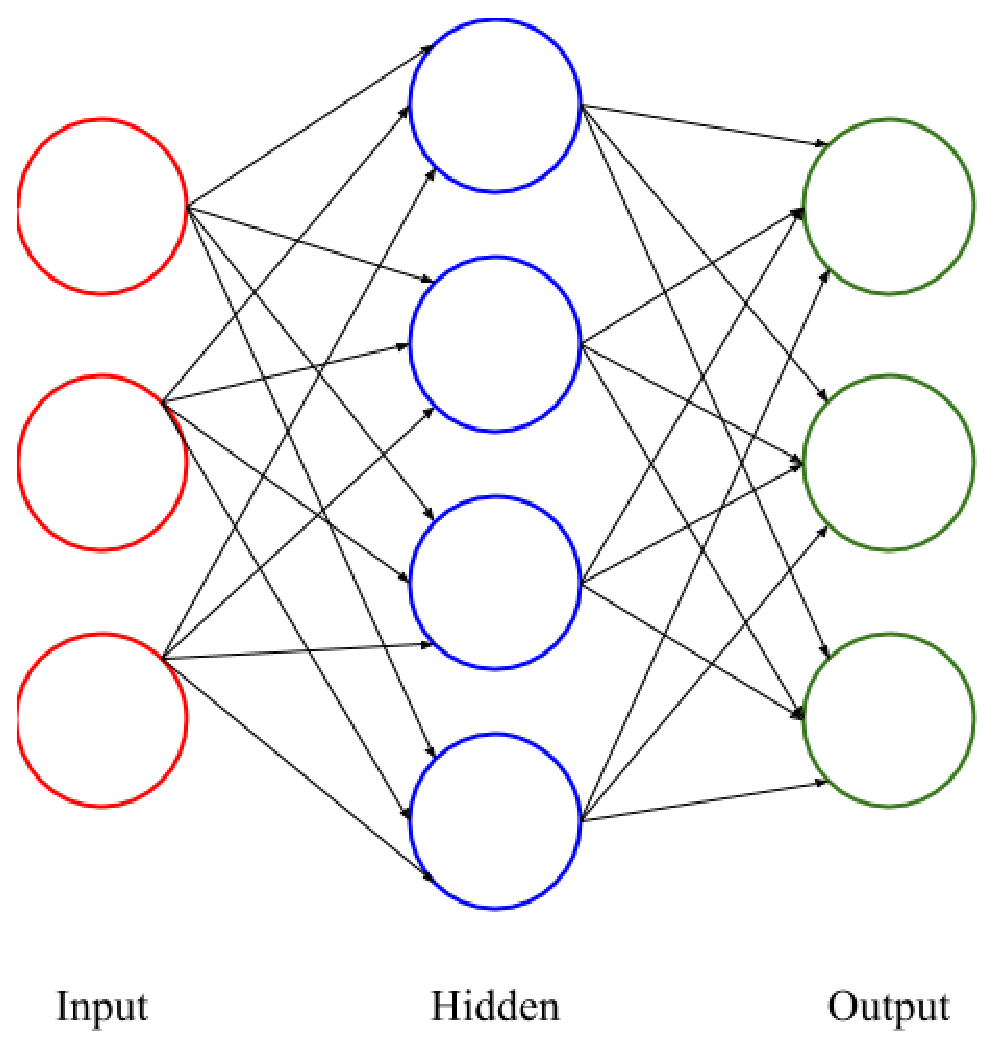
\includegraphics[height=2in]{../figures/neural_network.eps}
      \caption{Visualization of a fully-connected network.}
      \label{fig:nn}
    \end{figure} 
  \end{frame}

  \begin{frame}{Deep Neural Network}
    \begin{figure}[ht!]
      \centering
      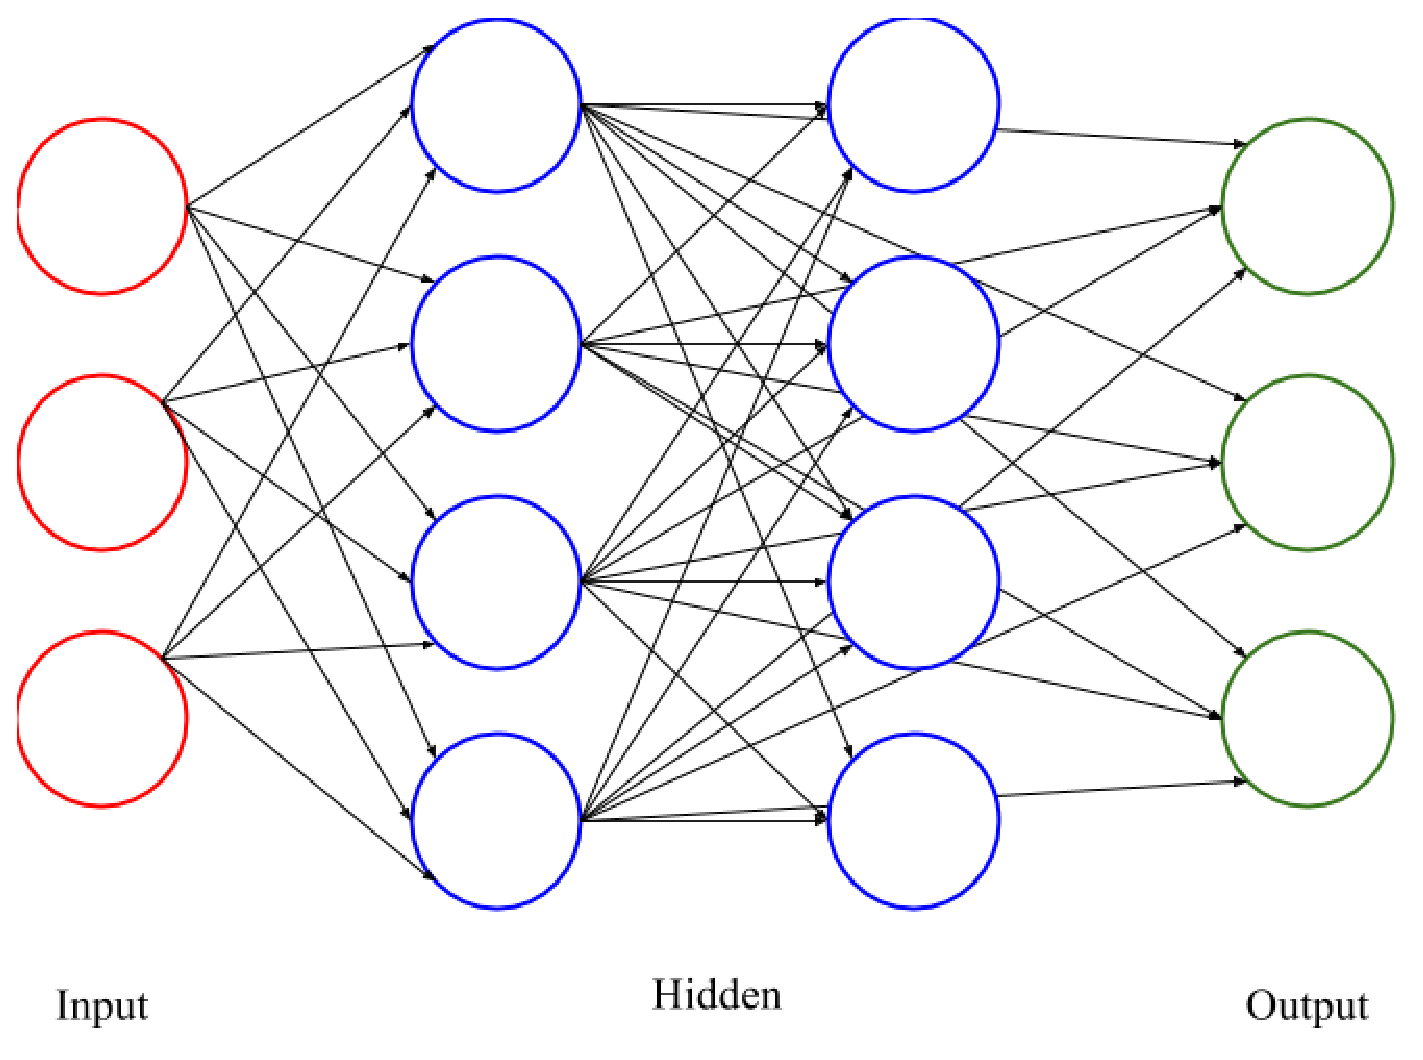
\includegraphics[height=2in]{../figures/deep_nn.eps}
      \caption{Visualization of a deep neural network}
      \label{fig:dnn}
    \end{figure}
  \end{frame}

  \begin{frame}{Convolutional Neural Network}
    \begin{figure}[ht!]
      \centering
      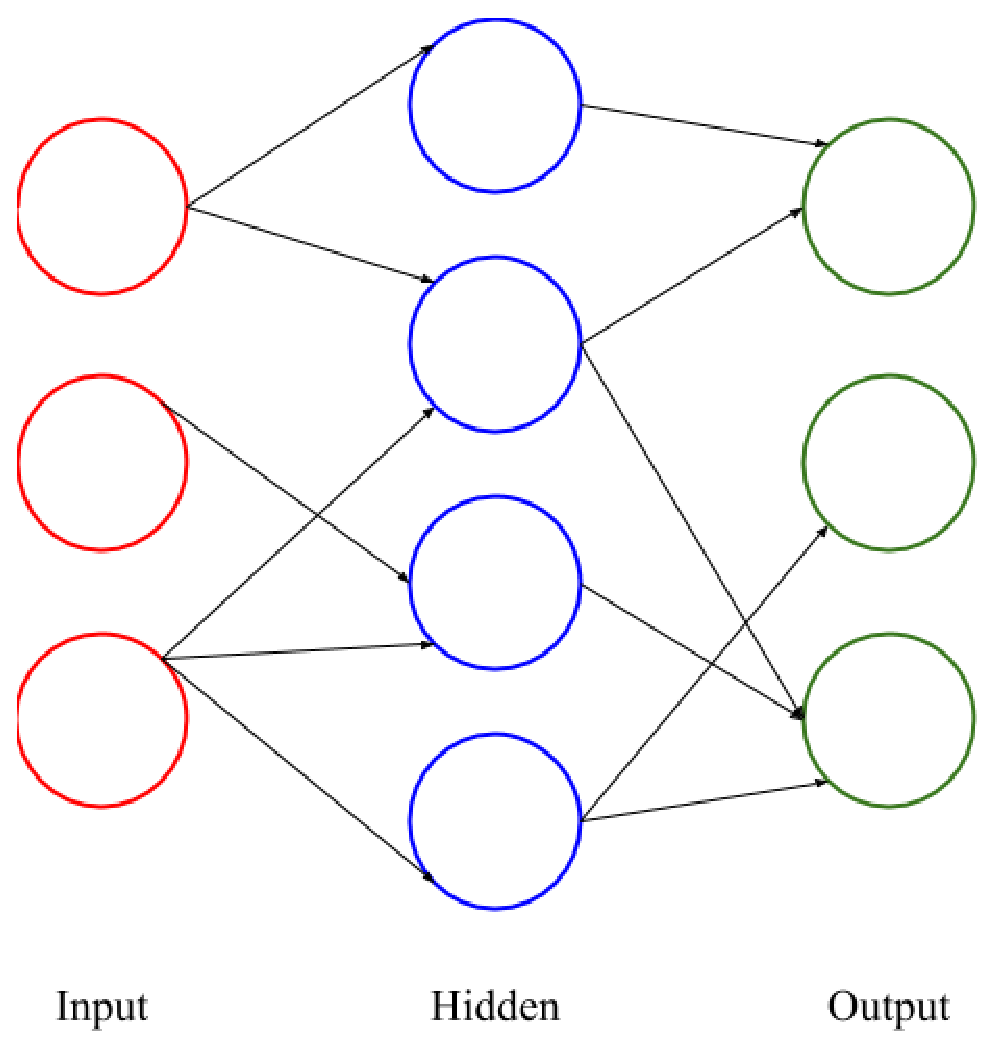
\includegraphics[height=2in]{../figures/convolutional_nn.eps}
      \caption{Visualization of a convolutional neural network}
      \label{fig:cnn}
    \end{figure}
  \end{frame}

  \begin{frame}{Datasets: MNIST}
    \begin{itemize}
      \item handwritten digit recognition
      \item 28x28 pixel, greyscale
      \item 60,000 training images, 10,000 testing images
    \end{itemize}
    \begin{center}
      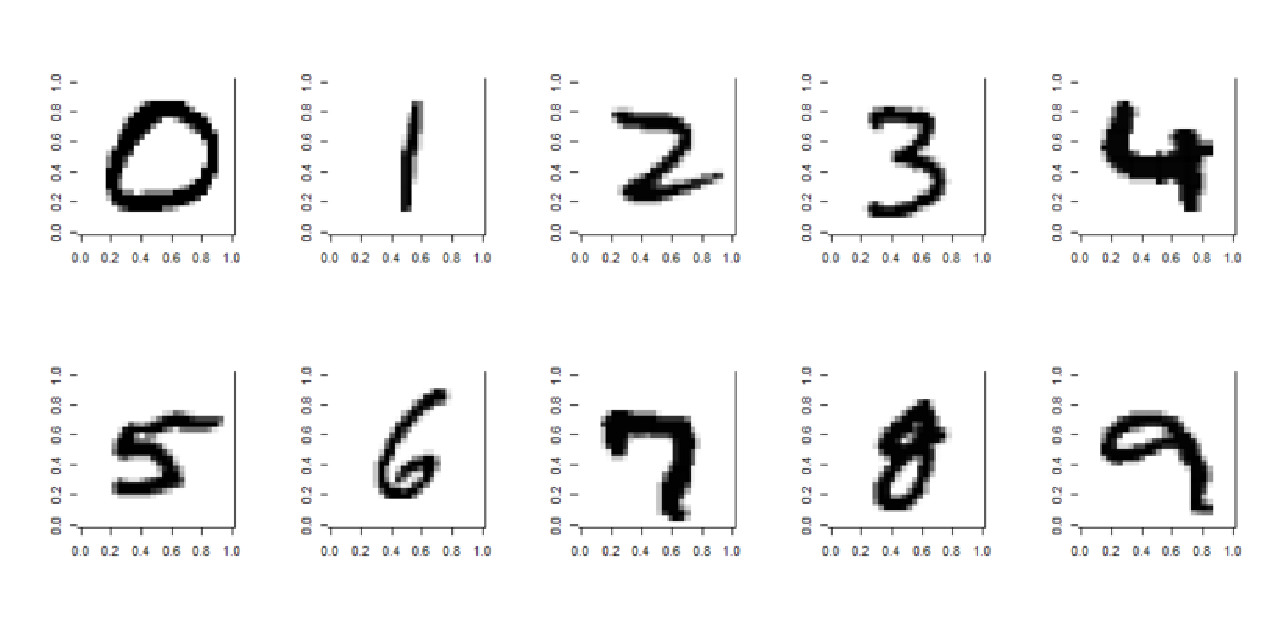
\includegraphics[height=2in]{../figures/mnist.eps}
    \end{center}
  \end{frame}

  \begin{frame}{Linear Classification}
    Essentially a 0-layer neural network\\
    Linear classification has two important parts:
    \begin{itemize}
      \item prediction function: maps data to class scores
      \item loss function: compares predicted scores with actual labels
    \end{itemize}
  \end{frame}

  \begin{frame}{Prediction Function}
    How likely is it that each training example is part of any class?
    $$ P = XW + b $$
    \begin{itemize}
      \item $X$: training data
      \item $W$: weights
      \item $b$: bias vector
    \end{itemize}
  \end{frame}

  \begin{frame}{Loss Function}
    Evaluates $P$ based on actual data labels
    $$ L = \sum_{i=1}^m L_i(P_i, y_i). $$
    \begin{itemize}
      \item $y$: labels for training data
      \item $L_i$: loss for one training example
      \item $L$: overall loss over entire training dataset
    \end{itemize}
  \end{frame}

  \begin{frame}{Softmax Loss Function}
    $$L(P) = -\frac{1}{m} \sum_{i=1}^m \log \frac{\exp{P_{i, y_i}}}
              {\sum_{j=1}^k \exp{P_{i, j}}}. $$
  \end{frame}

  \begin{frame}{Gradient Descent}
    Goal: find optimal $W$ and $b$ by minimizing $L$\\
    Steps of Gradient Descent:
    \begin{enumerate}
      \item forward propogation: \begin{itemize}
        \item calculate $P$
      \end{itemize}
      \item back propogation: \begin{itemize}
        \item calculate $\nabla P$
        \item use $\nabla P$ to calculate gradients w.r.t. model parameters
      \end{itemize}
      \item update $W$ and $b$ accordingly
    \end{enumerate}
  \end{frame}

  \begin{frame}{Deriving $\nabla P$}
    Goal: find $\frac{\partial L}{\partial W}$ and
    $\frac{\partial L}{\partial b}$ using Chain Rule.
    $$ L_i(P) = -\frac{1}{m} \left[ P_{i, y_i} - \log\left( \sum_{j=1}^k \exp
    P_{i, j} \right)\right] $$ for all $i$ where $1 \leq i \leq m$.

    $L_i$ depends on $P_{i, v}$ $\forall$ v $1 \leq v \leq k$,
    so $\frac{\partial L_i}{\partial P_{u, v}} = 0$ if $u \neq i$.

    $Y$: $m \times k$ where $Y_{i, j} = 1$ if $y_i == j$, and 0 otherwise.

  \end{frame}

  \begin{frame}{Deriving $\nabla P$}
    $$ \frac{\partial L_i}{\partial P_{i, v}} = -\frac{1}{m} Y_{i, v}
        + \frac{1}{m} \frac{exp(P_{i, v})}{\sum_{j=1}^k \exp P_{i, j}}$$.
    $$ \frac{\partial L}{\partial P_{i, v}} =
       \sum_{u=1}^m \frac{\partial L_u}{\partial P_{i, v}} =
       -\frac{1}{m} Y_{i, v} + \frac{1}{m} \frac{exp(P_{i, v})}{\sum_{j=1}^k
       \exp P_{i, j}}. $$

    $$ \nabla P_{i, v} = \frac{\partial L}{\partial P_{i, v}} \forall i, v.$$

    $$ \nabla P = \frac{1}{m} \left[ -Y + \frac{\exp P}{\sum_{j=1}^m \exp P_j}
       \right]. $$
  \end{frame}

  \begin{frame}{Deriving $\nabla W$}
    Facts:
    \begin{itemize}
      \item $P = XW + b$, meaning $P_{i, j} = \sum_{t=1}^n X_{i, t}W_{t, j} + b_j $
      \item $L_i$ is a function of $P_{u, v}$ only if $u = i$
      \item $\nabla P_{i, j} = \frac{\partial L}{\partial P_{i, j}} 
            = \frac{\partial L_i}{\partial P_{i, j}}$.
    \end{itemize}
  \end{frame}

  \begin{frame}{Deriving $\nabla W$}
    \begin{align*} 
         \frac{\partial L}{\partial W_{u, v}} = 
         \sum_{i=1}^m \frac{\partial L_i}{\partial W_{u, v}} &= 
         \sum_{i=1}^m \sum_{j=1}^k \frac{\partial L_i}{\partial P_{i, j}}
           \frac{\partial P_{i, j}}{\partial W_{u, v}}\\
         &= \sum_{i=1}^m \sum_{j=1}^k
             \frac{\partial L_i}{\partial P_{i, j}} X_{i, u}\\
         &= \sum_{i=1}^m \frac{\partial L_i}{\partial P_{i, v}} X_{i, u}\\ % confuse
         &= \sum_{i=1}^m \nabla P_{i, v} X_{i. u}\\
         &= \left( X^T \nabla P \right)_{u, v}.
    \end{align*}

  \end{frame}

  \begin{frame}{Deriving $\nabla W$}
    Recall: $$\frac{\partial L}{\partial W_{u, v}} =  \left( X^T \nabla P
    \right)_{u, v}.$$

    So:
    $$ \nabla W = X^T \nabla P. $$

    Similarly, we can show that
    $$ \nabla b = \sum_{j=0}^k P_j. $$
  \end{frame}

  \begin{frame}{Gradient Descent Update}
    Update $W$ and $b$:
    \begin{center}
      $$ W = W - \eta \nabla W, $$
      and
      $$ b = b - \eta \nabla b, $$
      where $\eta$ is the learning rate.
    \end{center}

  \end{frame}

  \begin{frame}{Single Layer Neural Network}
    Steps:
    \begin{enumerate}
      \item Forward propogation:
      \begin{enumerate}
        \item $ A = XW^{(1)} + b^{(1)} $
        \item $ Z = \phi(A) $
        \item $ P = ZW^{(2)} + b^{(2)} $
      \end{enumerate}

      \item Backward propogation:
      \begin{enumerate}
        \item calculate $\nabla W^{(1)}, \nabla W^{(2)}, \nabla b^{(1)},
              \nabla b^{(1)}, \nabla Z$
      \end{enumerate}
      \item Update weights:
        \begin{enumerate}
          \item e.g. $W^{(1)} = W^{(1)} - \eta \nabla W^{(1)}$
        \end{enumerate}
    \end{enumerate}

    where
    $$ \phi(x) = relu(x) =
      \begin{cases}
        0 & x < 0\\
        x & x \geq 0
      \end{cases}.$$
  \end{frame}

  \section{Demonstration}

  \section{Workflow}
  \begin{frame}{To Work On}
    Other Neural Network Architectures
    \begin{itemize}
      \item deep
      \item convolutional (if time allows)
    \end{itemize}
    Additional Neural Network features
    \begin{itemize}
      \item dropout % determines nodes to ignore - prevents overfitting
      \item batch normalization
    \end{itemize}
  \end{frame}

  \section{Thank-you!}
\end{document}
